\documentclass[9pt,aspectratio=169]{beamer}

\usetheme{graham}
% \beamertemplategridbackground[0.25cm]
\usepackage{luamplib}
\everymplib{input mpcolornames; beginfig(1);}
\everyendmplib{endfig;}

\title{Inclusion/Exclusion Principle}
\subtitle[Graham Middle School]{Graham Middle School Math Olympiad Team}

\begin{document}
\maketitle

\begin{frame}{Basic statistical terms}
  \begin{columns}[T]
    \begin{column}{0.5\textwidth}
      \begin{definition}
        The \textbf{average} (\textbf{arithmetic mean}) of a set of $N$ numbers is the sum of all $N$ numbers divided by $N$.\medskip
        
        The \textbf{mode} of a set of numbers is the number occurring \emph{most frequently} in the set.\medskip

        The \textbf{median} of an ordered set (from smallest to largest) of $N$ numbers is the \emph{middle number} if $N$ is odd, or the \emph{mean of the two middle numbers} if $N$ is even. \medskip

        The \textbf{range} of a set is a difference between the largest and the smallest elements.
      \end{definition}
      \vspace*{0.5em}
      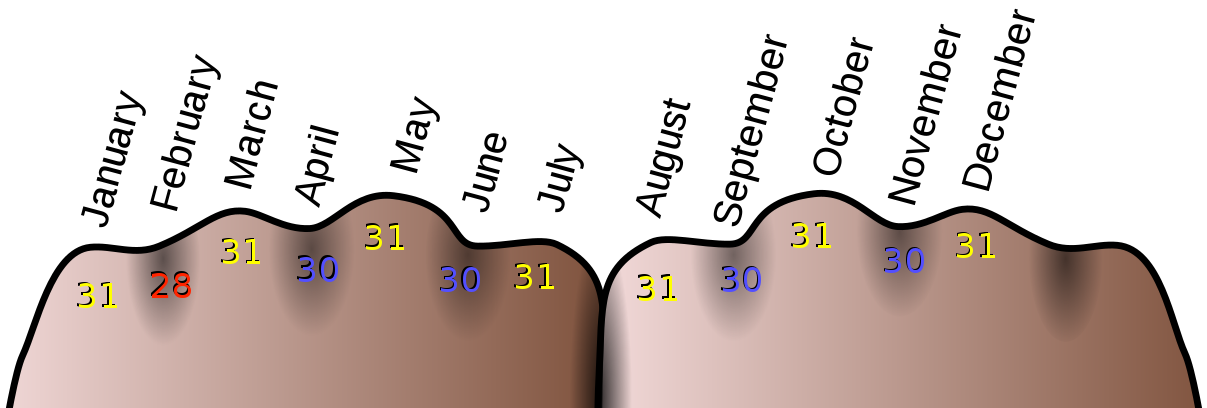
\includegraphics[width=\textwidth]{08 - Inclusion Exclusion Principle/hands.png}
    \end{column}
    \begin{column}{0.5\textwidth}
      Consider the set containing the number of days in each month of the year (non-leap year).  What are the mean, mode, and median for this set?

      The elements in this set are 
      \[ \left\{31, 28, 31, 30, 31, 30, 31, 31, 30, 31, 30, 31\right\}.\]
      
      To find mode and median it is useful to sort them
      \[ \left\{28, 30, 30, 30, 30, 31, 31, 31, 31, 31, 31, 31\right\}. \]
      $31$ occurs most frequently, so it is the \textbf{mode}. 
      
      The median is the mean of the 6\textsuperscript{th} and 7\textsuperscript{th} elements of the set (both of which are $31$), so the \textbf{median} is $31$.
      
      The \textbf{mean} is the sum of all numbers in the set $365$ divided by $12$, which is $30\, \dfrac{5\vphantom{5^5}}{12}$.\smallskip

      The range is difference between $31$ (the largest value) and $28$ (the smallest), so the \textbf{range} is $3$.
    \end{column}
  \end{columns}
\end{frame}

\begin{frame}{Sets}
  \begin{columns}[T]
    \begin{column}{0.5\textwidth}
      \begin{definition}
        In mathematics, a \textbf{set} is a \emph{collection} of elements.
      \end{definition}
      The elements that make up a set can be any kind of mathematical objects: numbers, symbols, points in space, lines, etc.  Sets are usually denoted as capital Latin letters.
      \begin{wrapfigure}[5]{r}{0.35\textwidth}
        \vspace*{-1.7em}
        \begin{mplibcode}
          u=0.4cm;
          path a, b, aa, ab, c;
          a = fullcircle scaled 3u;
          b = a shifted (0, -1.7u);
          c = a shifted (3.5u, -1.3u);
          ab = buildcycle(a, b);
          fill a withcolor 0.8[red, white];
          fill b withcolor 0.7[rgb_yellow, white];
          fill ab withcolor 0.5[0.5[rgb_yellow, red], white];
          fill c withcolor 0.8[green, white];
          draw a;
          draw b;
          draw c;
          label.(btex $1$ etex, (0u, -0.85u));
          label.(btex $2$ etex, (-0.7u, 0.4u));
          label.(btex $3$ etex, (2.4u, 0.8u));
          label.(btex $4$ etex, (2.9u, -1.05u));
          label.(btex $5$ etex, (0.6u, 0.6u));
          label.(btex $6$ etex, (0u, -2.3u));
          label.(btex $7$ etex, (4u, -1.55u));
        \end{mplibcode}
      \end{wrapfigure}
      Sometimes it is helpful to visualize sets as circles with all their elements inside.

      For example, this diagram represents $3$ sets: the red set with elements $2$, $5$, and $1$, the yellow set with elements $1$ and $6$, and the green with elements $4$ and $7$. $3$ doesn't belong to any set. If we denote the sets as $R$, $Y$ and $G$, we can write
      \[ R = \left\{1, 2, 5\right\},\ \  Y = \left\{1, 6\right\}\ \ \text{and}\ \ G = \left\{4, 7\right\}. \]
      \vspace*{-0.9\baselineskip}
      \begin{definition}
        The \textbf{number} of elements (the set \emph{cardinality}) in a~set $S$ is denoted as $|S|$.
      \end{definition}
      \vspace*{-1\baselineskip}
      \[|R| = 3,\quad  |Y| = 2,\quad  |G| = 2.\]
    \end{column}
    \begin{column}{0.5\textwidth}
      \begin{definition}
        The \textbf{union} (denoted by $\cup$) of sets is the set of all elements in \emph{any} of this set.
      \end{definition}
      For example
      \[ R \cup Y = \left\{1, 2, 5, 6\right\},\quad  Y \cup G = \left\{1, 4, 6, 7\right\}. \]
      \vspace*{-0.9\baselineskip}
      \begin{definition}
        The \textbf{intersection} (denoted by $\cap$) of sets is the set whose elements are in \emph{all} sets.
      \end{definition}
      For example
      \[ R \cap Y = \left\{1\right\},\quad  Y \cap G = \left\{\ \right\} = \varnothing. \] 
      The symbol $\varnothing$ denotes the \textbf{empty set}, the set without elements.
      \begin{definition}
        \vspace*{-0.3em}
        The \textbf{complement} of a set $S$ (denoted as $S'$ or $\overline{S}$) is a set of all elements \emph{not in} a set $S$.
      \end{definition}
      For example if we consider only elements from $1$ to $7$ (it is also called an \textbf{universal set})
      \[ R′ = \left\{3, 4, 6, 7\right\},\quad  G′ = \left\{1, 2, 3, 5, 6\right\}. \]
    \end{column}
  \end{columns}
\end{frame}

\begin{frame}{Inclusion/Exclusion Principle}
  \begin{columns}[T]
    \begin{column}{0.5\textwidth}
      \begin{problem}
        What the number of integers less than or equal to $100$ that were factors of $4$ or factors of $5$?
      \end{problem}
      We knew there were $25$ factors of $4$ and $20$ factors of $5$, but the final answer was 
      \[ 25 + 20 - 5 = 40, \]
      because we had to subtract the $5$ factors of $20$ that were being counted twice.

      We can generalize this to the counting of elements in any two sets $A$ and $B$.
      \vspace*{-0.9\baselineskip}
      \begin{columns}[totalwidth=0.8\textwidth]
        \begin{column}{0.45\textwidth}
          \begin{center}
            \leavevmode
            \begin{mplibcode}
              u=0.45cm;
              path a, b;
              a = fullcircle scaled 3u;
              b = a shifted (1.85u, 0);
              draw a;
              draw b;
              label.(btex $1$ etex, (-0.5u, 0u));
              label.(btex $1$ etex, (2.35u, 0u));
              label.(btex $2$ etex, (0.925u, 0u));
              label.(btex $A$ etex, (-1.7u, 1.1u));
              label.(btex $B$ etex, (3.55u, 1.1u));
            \end{mplibcode}
            \[ |A| + |B| \]
          \end{center}
        \end{column}
        \begin{column}{0.45\textwidth}
          \begin{center}
            \leavevmode
            \begin{mplibcode}
              u=0.45cm;
              path a, b;
              a = fullcircle scaled 3u;
              b = a shifted (1.85u, 0);
              draw a;
              draw b;
              label.(btex $1$ etex, (-0.5u, 0u));
              label.(btex $1$ etex, (2.35u, 0u));
              label.(btex $1$ etex, (0.925u, 0u));
              label.(btex $A$ etex, (-1.7u, 1.1u));
              label.(btex $B$ etex, (3.55u, 1.1u));
            \end{mplibcode}
            \[ |A| + |B| - |A \cap B| \]
          \end{center}
        \end{column}
      \end{columns}
      \vspace*{-0.5\baselineskip}
      The numbers in the diagram above indicate how many times the elements in each region are counted.
    \end{column}
    \begin{column}{0.5\textwidth}
      Where $A$ and $B$ overlap, elements are counted twice. 
      \begin{definition}
        Therefore to find the number of the elements in $A$ and $B$, we must subtract the number of the elements present in both sets. 
        \[ |A \cup B| = |A| + |B| - |A \cap B|. \]
        \vspace*{-0.9\baselineskip}
      \end{definition}
      \begin{problem}
        There are $12$ cookies with chocolate chips, and $10$ cookies with nuts.  If there are $4$ cookies with chips and nuts, how many cookies are there?
      \end{problem}
      To find the total number of cookies, we sum the cookies from each category ($12 + 10$), and then subtract the cookies that overlap both categories ($4$) to find the total is $18$.
    \end{column}
  \end{columns}
\end{frame}

\begin{frame}{Inclusion/Exclusion Principle Extended}
  \begin{columns}[T]
    \begin{column}{0.5\textwidth}
      This counting principle for overlapping sets can be extended to $3$ sets.
      
      The diagram below shows $3$ overlapping sets and the numbers labeling each region indicate how many times that region is counted in the operation shown beneath it.  To find the total number of elements, we must count the elements in each set, then subtract the elements for the $3$ pairwise intersections, and finally add back the elements found in all $3$ sets.

      \vspace*{-0.9\baselineskip}
      {\tiny
      \begin{columns}[totalwidth=1\textwidth]
        \begin{column}{0.33\textwidth}
          \begin{center}
            \leavevmode
            \begin{mplibcode}
              u=0.3cm;
              path a, b, c;
              a = fullcircle scaled 3u;
              b = a shifted (1.85u, 0);
              c = a shifted (0.925u, -1.6u);
              draw a;
              draw b;
              draw c;
              label.(btex $1$ etex, (-0.5u, 0.3u));
              label.(btex $1$ etex, (2.35u, 0.3u));
              label.(btex $1$ etex, (0.925u, -2.1u));
              label.(btex $2$ etex, (0.925u, 0.4u));
              label.(btex $2$ etex, (0.2u, -0.9u));
              label.(btex $2$ etex, (1.7u, -0.9u));
              label.(btex $3$ etex, (0.925u, -0.55u));
              label.(btex $A$ etex, (-1.7u, 1.1u));
              label.(btex $B$ etex, (3.55u, 1.1u));
              label.(btex $C$ etex, (2.55u, -3u));
            \end{mplibcode}
            \begin{multline*}
              |A| + |B| + |C|
            \end{multline*} 
          \end{center}
        \end{column}
        \begin{column}{0.33\textwidth}
          \begin{center}
            \leavevmode
            \begin{mplibcode}
              u=0.3cm;
              path a, b, c;
              a = fullcircle scaled 3u;
              b = a shifted (1.85u, 0);
              c = a shifted (0.925u, -1.6u);
              draw a;
              draw b;
              draw c;
              label.(btex $1$ etex, (-0.5u, 0.3u));
              label.(btex $1$ etex, (2.35u, 0.3u));
              label.(btex $1$ etex, (0.925u, -2.1u));
              label.(btex $1$ etex, (0.925u, 0.4u));
              label.(btex $1$ etex, (0.2u, -0.9u));
              label.(btex $1$ etex, (1.7u, -0.9u));
              label.(btex $0$ etex, (0.925u, -0.55u));
              label.(btex $A$ etex, (-1.7u, 1.1u));
              label.(btex $B$ etex, (3.55u, 1.1u));
              label.(btex $C$ etex, (2.55u, -3u));
            \end{mplibcode}
            \begin{multline*}
              |A| + |B| + |C| - {}\\
              {} - |A \cap B| - |A \cap C| - {} \\ 
              {} - |B \cap C|
            \end{multline*} 
          \end{center}
        \end{column}
        \begin{column}{0.33\textwidth}
          \begin{center}
            \leavevmode
            \begin{mplibcode}
              u=0.3cm;
              path a, b, c;
              a = fullcircle scaled 3u;
              b = a shifted (1.85u, 0);
              c = a shifted (0.925u, -1.6u);
              draw a;
              draw b;
              draw c;
              label.(btex $1$ etex, (-0.5u, 0.3u));
              label.(btex $1$ etex, (2.35u, 0.3u));
              label.(btex $1$ etex, (0.925u, -2.1u));
              label.(btex $1$ etex, (0.925u, 0.4u));
              label.(btex $1$ etex, (0.2u, -0.9u));
              label.(btex $1$ etex, (1.7u, -0.9u));
              label.(btex $1$ etex, (0.925u, -0.55u));
              label.(btex $A$ etex, (-1.7u, 1.1u));
              label.(btex $B$ etex, (3.55u, 1.1u));
              label.(btex $C$ etex, (2.55u, -3u));
            \end{mplibcode}
            \begin{multline*}
              |A| + |B| + |C| - {}\\
              {} - |A \cap B| - |A \cap C| - {} \\ 
              {} - |B \cap C| + | A \cap B \cap C|
            \end{multline*} 
          \end{center}
        \end{column}
      \end{columns}
      }
      \vspace*{-0.5\baselineskip}
      Again, the numbers in the diagrams above indicate how many times the elements in each region are counted. 
    \end{column}
    \begin{column}{0.5\textwidth}
      \begin{problem}
        There are $12$ cookies with chocolate chips, $18$ cookies with nuts, and $8$ cookies with raisins.  If there are $8$ cookies with chips and nuts, $2$ cookies with chips and raisins, $8$ cookies with raisins and nuts, and $2$ cookies with chips, nuts, and raisins, how many cookies are there in total?
      \end{problem}
      Using the overlapping counting principle:
      \begin{align*}
        \text{chips} + \text{nuts} + \text{raisins} &= 38, \\
        \text{chips/nuts} + \text{chips/raisins} + \text{nuts/raisins} &= 18, \\
        \text{chips/nuts/raisins} &= 2, \\
        \text{Total number of cookies} = 38 - 18 + 2 &= 22.
      \end{align*}
      \begin{center}
        \vspace*{-\baselineskip}
        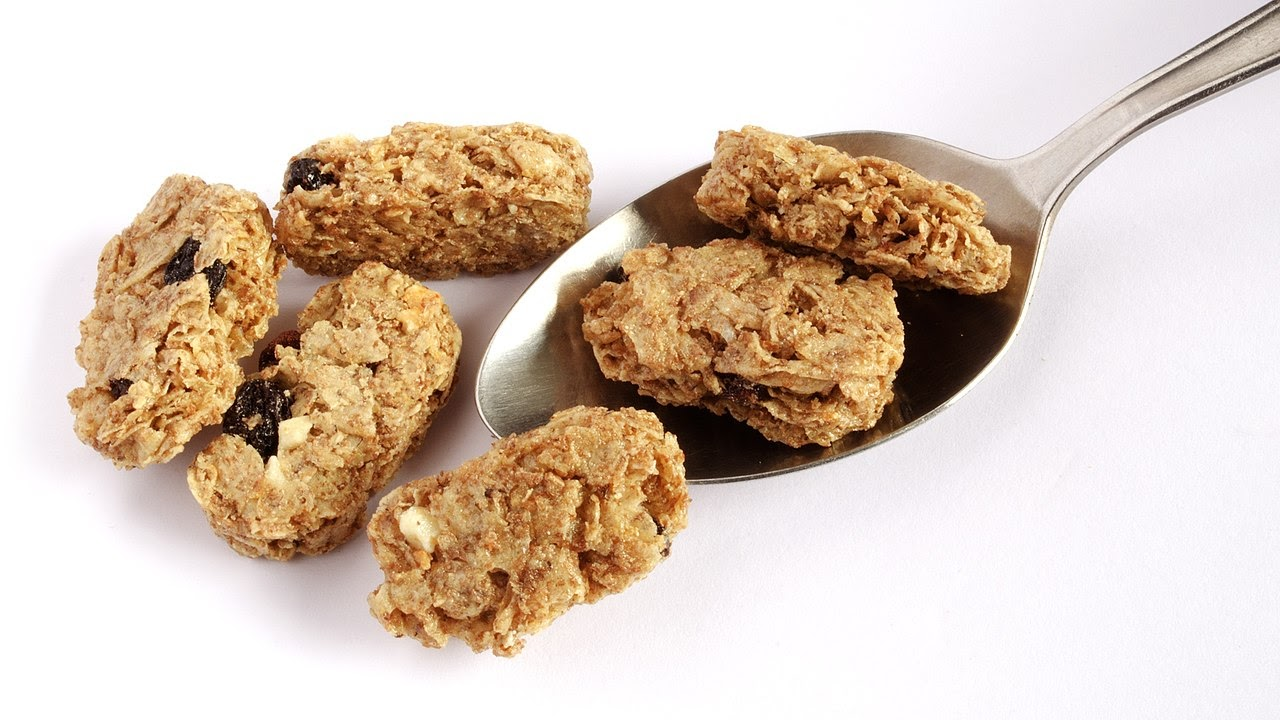
\includegraphics[width=0.6\textwidth]{08 - Inclusion Exclusion Principle/cookies.jpg}
      \end{center}
    \end{column}
  \end{columns}
\end{frame}

\begin{frame}{Casework}
  \begin{columns}[T]
    \begin{column}{0.5\textwidth}
      \begin{definition}
        Casework is a counting method where you divide a problem into \emph{several groups} based on some property (known as cases), count these cases individually, and then sum the totals from each case. Casework is a very general problem solving approach, and is used a tremendous amount in middle school math contests.  Be careful of potential case overlap. 
        
        \emph{If the same solution occurs in two of your cases, don’t count it twice.}
      \end{definition}
      \small
      \begin{problem}
        How many pairs of positive integers $(x, y)$ satisfy the equation $x^4 + y < 70$?
      \end{problem}
      \textbf{Case 1}: $x = 1$.  $1 + y < 70$.  So $0 < y < 69$, and there are $68$ possible pairs $(1,\ 1)$, $(1,\ 2)$, $\ldots$, $(1,\ 68)$.
      
      \textbf{Case 2}: $x = 2$.  $16 + y < 70$.  So $0 < y < 54$, and there are $53$ possible pairs $(2,\ 1)$, $(2,\ 2)$, $\ldots$, $(2,\ 53)$.

      Note $3^4 = 81$, so there are only two cases to consider ($x = 1 \text{ or } 2$) with no overlap between them.
      \[ \text{Total pairs} = 68 + 53 = 121. \]
    \end{column}
    \begin{column}{0.5\textwidth}
      \small
      \begin{problem}
        There are a $3$ distinct urns (containers $A$, $B$, $C$) and $4$ identical balls.  I need the put all of the balls into the urns, and I am free to place $0-4$ balls into any urn.  How many distinct ways are there to put the balls into the urns?
      \end{problem}
      \textbf{Case 1}:  All $4$ balls in a single urn -- \textbf{$3$ ways}.
      
      \textbf{Case 2}: $3$ in one urn, $1$ in a different urn.  There are $3$ choices for the urn with $3$ balls, and then $2$ choices remaining for the urn with the single ball, so there are $3 \times 2 = 6$ \textbf{ways}.
      
      \textbf{Case 3}: $2$ balls in one urn, and $2$ balls in a different urn.  It is $6$ arrangements ($3$ ways to pick the first urn, and then $2$ ways to pick the second urn), and because $2$ balls first into urn $A$ and then $2$ balls into urn $B$ is the same if we swap urns $A$ and $B$, we need to divide by $2$. So the answer is $\frac{3 \times 2}{2} = 3$ \textbf{ways}.
      
      \textbf{Case 4}: $2$ balls in one urn, and one ball in each of the other urns.  There are $3$ choices for the urn with $2$ balls.  There is no other flexibility to choose, since one ball must occupy each of the other $2$ urns.  So $3$ \textbf{ways} for this case.\smallskip
      
      Therefore there are $3 + 6 + 3 + 3 = 15$ \textbf{ways} to arrange the balls into urns.
    \end{column}
  \end{columns}
\end{frame}

\begin{frame}{Stars and bars}
  \begin{columns}[T]
    \begin{column}{0.5\textwidth}
      Going through the casework for the simple case of $4$ balls and $3$ urns was time-consuming, and would become impossible to do without a computer as the numbers grow larger.  There is, however, a technique that can be used to solve such problems.  We will represent each ball by a~star $\star$, and the boundary between urns by a~vertical bar $\mid$.  Any star to the left of the first bar is in urn $A$, any star between the pair of bars is in urn $B$, and any stars to the right of second bar is in urn $C$.  So \small{\fbox{$\star\mid\star\,\star\mid\star$}} can be read as $1$ ball in urn~$A$, $2$ balls in urn $B$ and $1$ ball in urn $C$.  The $15$ arrangements from the $4$ cases on the previous slide are:
      \small
      \begin{example}
        Case 1: \fbox{$\star\star\star\,\star\mid\,\mid$}, \fbox{$\mid\star\star\star\,\star\mid$}, \fbox{$\mid\,\mid\star\star\star\,\star$}.
        
        Case 2: \fbox{$\star\star\star\mid\star\mid$}, \fbox{$\star\star\star\mid\,\mid\star$}, \fbox{$\star \mid\star\star\star\mid$},\\
        \hphantom{Case 2:} \fbox{$\mid\star\star\star\mid\star$}, \fbox{$\star\mid\,\mid\star\star\star$}, \fbox{$\mid\star\mid\star\star\star$}.
        
        Case 3: \fbox{$\star\,\star\mid\star\,\star\mid$}, \fbox{$\star\,\star\mid\,\mid\star\,\star$}, \fbox{$\mid\star\,\star\mid\star\,\star$}.

        Case 4: \fbox{$\star\,\star\mid\star\mid\star$}, \fbox{$\star\mid\star\,\star\mid\star$}, \fbox{$\star\mid\star\mid\star\,\star$}.
      \end{example}
    \end{column}
    \begin{column}{0.5\textwidth}
      \begin{definition}
        If we have $k$ balls and $n$ urns, we can represent them with a row of $k$ stars and $n - 1$ bars ($n - 1$ bars separate the stars into regions to represent the $n$ urns).  
      \end{definition}

      Using our combinatorics knowledge, we can figure out how many distinct ways there are to arrange a row of identical star and bar symbols. 

      There are 
      \[ \frac{(n + k - 1)!}{k! \times (n - 1)!} \]
      distinct arrangements.  This fraction is equivalent to $C^{n + k - 1}_k$.  We divide the $(n + k - 1)!$ permutations by $k!$ because there are $k$ indistinguishable stars to arrange, and by $(n - 1)!$ because there are $n - 1$ identical bars to arrange.  So for the $4$ balls and $3$ urns, there should be $C^6_4 = 15$ arrangements.
    \end{column}
  \end{columns}
\end{frame}

\begin{frame}{Stars and bars example}
  \begin{columns}[T]
    \begin{column}{0.5\textwidth}
      This was Problem 25 (the final and allegedly hardest) question on the AMC 8 in 2019.  It is not really possible to solve this problem with casework due to time constraints on the exam, but seeing how we can apply "Stars and Bars" makes it computationally simple.
      \begin{problem}
        Alice has $24$ apples.  In how many ways can she share them with Ben and Chris so that each of the three people has at least two apples?
      \end{problem}

      The $24$ apples are identical in terms of counting, so they can be thought of as the "Stars".  Each person is the destination for the apple, so they are the $3$ urns (meaning we have 2 "Bars").  There is an added complication, in that each person must have at least $2$ apples.  No problem.  Just subtract these $6$ apples from the $24$, and Alice must now split $18$ apples ($k = 18$) into $3$ groups ($n = 3$).  This is $C^{20}_{18} = 190$.

    \end{column}
    \begin{column}{0.5\textwidth}
      \begin{center}
        \vspace*{-1\baselineskip}
        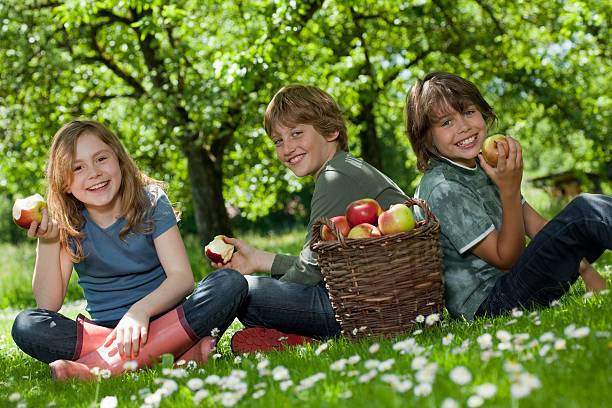
\includegraphics[width=\textwidth]{08 - Inclusion Exclusion Principle/apples.jpg}
      \end{center}
      Transforming a counting problem into a combinations calculation is possible here because we see that it’s equivalent to arranging a pattern consisting of only two types of symbols: stars and bars.
    \end{column}
  \end{columns}
\end{frame}

\begin{frame}{Exercises}
  \begin{columns}[T]
    \begin{column}{0.5\textwidth}
      \begin{enumerate}
        \item What is the smallest possible average of four distinct positive even integers?
        \item In a gymnastics competition, judge’s marks are integers $0-10$ inclusive.  There are $6$ judges, and the athlete's score is calculated by taking the average of the remaining $4$ marks after the highest and lowest marks are eliminated.  The winning gymnast had a $8.5$ score, while the second place finisher had a $8.0$ score.  If the both received identical lowest marks, could the highest marks they received have changed the order of finish if they were included in the scoring average?  Explain your reasoning.
        \item The \emph{harmonic} mean of a set of non-zero numbers is the reciprocal of the average of the reciprocals of the numbers. 
        What is the harmonic mean of $1$, $2$, and $4$?
        \seti
      \end{enumerate}
    \end{column}
    \begin{column}{0.5\textwidth}
      \begin{enumerate}
        \conti
        \item What is median of the following data set:\\ $2$, $3$, $3$, $4$, $4$, $4$?
        \item In school's band string section, $28$ students play the violin, $18$ students play the viola, and $12$ students play both.  How many students are in the string section?
        \item There are $25$ students in a class. $12$ of them are on a football team and $14$ are on a soccer team. If $3$ students are on neither of these teams, how many students are on both the football and soccer teams?
        \item How many integer pair $(x, y)$ solutions are there to $x^2 + y^2 < 10$?
        \item If there are breakout rooms to work on $4$ different types of math problems, how many ways are there to split $20$ students into the breakout rooms, if each breakout room must contain at least $3$ students?
      \end{enumerate}
    \end{column}
  \end{columns}
\end{frame}

\begin{frame}{Challenge problems}
  \begin{columns}[T]
    \begin{column}{0.5\textwidth}
      \begin{enumerate}
        \item The Girl Scouts sold boxes of cookies outside of the school one morning.  If they sold $252$ boxes of cookies to $100$ customers (and every customer bought at least one box of cookies), what is the maximum possible median number of boxes of cookies bought that morning?
        \item In Graham Middle School's woodwind section, $21$ students play clarinet, $16$ students play oboe, $13$ students play saxophone, $6$ students play clarinet and oboe, $5$ students play clarinet and saxophone, $4$ students play oboe and saxophone.  If there are $37$ students total in the woodwind section, how many play all $3$ instruments?
        \item How many distinct positive integer triplets $(x, y, z)$ are solutions to $x + y + z = 12$?
        \seti
      \end{enumerate}
    \end{column}
    \begin{column}{0.5\textwidth}
      \begin{enumerate}
        \conti
        \item When a fair $6$-sided die is rolled $7$ times, the probability that sum of the $7$ rolls will be $10$ can be represented as $\dfrac{n}{67}$.  Find the value of~$n$.
      \end{enumerate}
    \end{column}
  \end{columns}
\end{frame}

% \begin{frame}{Title}
%   \begin{columns}[T]
%     \begin{column}{0.5\textwidth}
%     \end{column}
%     \begin{column}{0.5\textwidth}
%     \end{column}
%   \end{columns}
% \end{frame}

\end{document}
